% Pacchetti richiesti nel preambolo del main.tex per la corretta compilazione di questo capitolo:
% \usepackage{tikz}
% \usetikzlibrary{shapes.geometric, positioning, arrows.meta, calc, decorations.pathreplacing}
% \usepackage{listings}
% \usepackage{amsmath}
% \usepackage{amssymb}

\chapter{Gestione delle Transazioni}

\section{Introduzione all'Affidabilità e alla Gestione delle Basi di Dati}

Le basi di dati costituiscono una risorsa fondamentale e critica per chi le possiede, rappresentando spesso il nucleo informativo essenziale per il funzionamento di aziende e organizzazioni. Per tale motivo, esse devono essere intrinsecamente affidabili e i dati in esse contenuti devono essere rigorosamente conservati, preservandone l'integrità anche e soprattutto in presenza di malfunzionamenti hardware o software, cadute di sistema (crash) o interruzioni anomale dell'alimentazione.

Un esempio classico che illustra la necessità critica di questa affidabilità è rappresentato dal trasferimento di fondi tra due conti correnti bancari. Questa operazione logica si scompone fisicamente in almeno due operazioni distinte: il prelievo dal primo conto e il successivo versamento sul secondo. Qualora si verificasse un guasto del sistema esattamente a metà dell'esecuzione, ovvero dopo il prelievo ma prima del versamento, la base di dati verrebbe a trovarsi in uno stato inconsistente, con una perdita netta di denaro.

Per prevenire simili anomalie, è strettamente necessario che i Sistemi di Gestione delle Basi di Dati (DBMS) forniscano un supporto nativo alla gestione di transazioni che godano di due proprietà fondamentali:
\begin{itemize}
    \item \textbf{Atomicità}: Le transazioni devono essere eseguite seguendo la logica del "tutto o niente" (all-or-nothing). Questo implica che le operazioni che compongono una transazione non possono essere applicate in modo parziale; o tutte le modifiche vengono riflesse nel database, oppure nessuna di esse deve avere alcun effetto, riportando il sistema allo stato antecedente l'inizio della transazione.
    \item \textbf{Definitività}: Le transazioni completate con successo devono produrre effetti definitivi. Dopo la loro naturale e corretta conclusione, le modifiche apportate divengono permanenti e il sistema non può in alcun modo "dimenticarle", a prescindere dai guasti futuri che potrebbero verificarsi.
\end{itemize}

Il raggiungimento e il mantenimento di tale affidabilità rappresentano una sfida tecnologica particolarmente impegnativa per l'architettura di un DBMS. Le basi di dati, infatti, non sono entità statiche, ma subiscono aggiornamenti continui e frequenti. In aggiunta, per questioni di efficienza e latenza, le operazioni di lettura e scrittura non avvengono direttamente sul disco fisico, ma passano attraverso un'area di memoria volatile, gestita dal modulo del sistema noto come gestore del buffer (buffer manager). La presenza di questo buffer introduce una complessità notevole: poiché i dati modificati nel buffer potrebbero non essere ancora stati trascritti fisicamente (flushed) sulla memoria secondaria al momento di un guasto, il sistema deve disporre di meccanismi avanzati per garantire che nessuna transazione confermata vada perduta e che nessuna transazione incompleta lasci tracce permanenti.

\section{Condivisione delle Risorse e Controllo della Concorrenza}

Oltre all'affidabilità, una caratteristica peculiare delle basi di dati è la loro natura profondamente condivisa. Una base di dati si configura come una risorsa integrata, destinata a essere fruita contemporaneamente da svariate applicazioni e utenti. Questa architettura multi-utente e multi-applicazione genera due ordini di conseguenze cruciali:
\begin{enumerate}
    \item \textbf{Meccanismi di autorizzazione}: Poiché vi sono attività diverse che insistono su dati parzialmente condivisi, è imperativo implementare sistemi di controllo degli accessi. Il DBMS deve assicurare che ogni utente o applicazione operi esclusivamente all'interno dei privilegi e dei permessi a esso accordati.
    \item \textbf{Controllo della concorrenza}: L'esecuzione simultanea di attività multi-utente su dati condivisi impone la necessità di orchestrare gli accessi concorrenti per evitare interferenze distruttive.
\end{enumerate}

Per comprendere la criticità del controllo della concorrenza, si considerino le problematiche derivanti da aggiornamenti simultanei su basi di dati condivise. Un primo esempio emblematico riguarda l'esecuzione di due prelevamenti che avvengono in modo (quasi) contemporaneo sul medesimo conto corrente da due sportelli bancomat differenti. Se il sistema leggesse per entrambe le operazioni il saldo iniziale prima di applicare la rispettiva detrazione, il saldo finale rifletterebbe l'aggiornamento di una sola transazione, "sovrascrivendo" e vanificando di fatto l'altra (fenomeno noto come \textit{lost update}). Un secondo esempio è fornito dai sistemi di biglietteria elettronica, dove due prenotazioni (quasi) contemporanee potrebbero tentare di riservare lo stesso identico posto su un volo o per uno spettacolo.

Intuitivamente, la soluzione più banale per garantire la correttezza assoluta delle transazioni consisterebbe nell'imporre una esecuzione strettamente seriale: elaborare la prima transazione per intero e, solo alla sua conclusione, avviare la seconda. Tuttavia, nei sistemi reali operanti su larga scala, forzare un'esecuzione puramente seriale penalizzerebbe l'efficienza e il throughput (il numero di transazioni eseguite per unità di tempo) in maniera del tutto inaccettabile, causando lunghi tempi di attesa. Pertanto, i DBMS implementano sofisticati meccanismi di controllo della concorrenza che permettono un ragionevole compromesso: essi consentono un'esecuzione "intrecciata" (interleaved) delle operazioni, ma esclusivamente quando questa sovrapposizione è sicura, garantendo che il risultato finale sia sempre logicamente equivalente a quello che si otterrebbe con una qualche esecuzione seriale.

\section{Architettura e Moduli di un DBMS}

La gestione delle transazioni coinvolge un ecosistema di moduli all'interno dell'architettura di un Sistema di Gestione di Basi di Dati. Il diagramma seguente illustra la scomposizione logica e l'interazione tra i gestori che si occupano dell'accesso ai dati, delle interrogazioni e dell'affidabilità transazionale.

\vspace{1em}
\begin{center}
\begin{tikzpicture}[
    node distance=0.8cm and 1.5cm,
    box/.style={draw, rectangle, minimum height=1cm, text width=4cm, align=center, fill=gray!10},
    db/.style={draw, cylinder, shape border rotate=90, aspect=0.25, minimum height=1.5cm, minimum width=2.5cm, align=center, fill=gray!20},
    arrow/.style={-{Stealth}, thick}
]

% Livello 1
\node[box, text width=6cm] (gestore_interr) {Gestore degli accessi e\\delle interrogazioni};
\node[box, right=of gestore_interr, text width=4cm] (gestore_trans) {Gestore\\delle transazioni};

% Livello 2
\node[box, below left=of gestore_interr.south, anchor=north] (gestore_agg) {Gestore di\\Interrogazioni e aggiornamenti};
\node[box, right=0.5cm of gestore_agg] (gestore_metodi) {Gestore dei\\metodi d'accesso};

\node[box, below right=of gestore_trans.south, anchor=north] (gestore_affid) {Gestore della\\affidabilità};
\node[box, left=0.5cm of gestore_affid] (gestore_conc) {Gestore della\\concorrenza};

% Livello 3
\node[box, below=1.5cm of gestore_metodi] (gestore_buffer) {Gestore\\del buffer};
\node[box, below=1.5cm of gestore_conc] (gestore_mem) {Gestore della\\memoria secondaria};

% Livello 4 (DB)
\node[db, below=1cm of gestore_mem] (memoria) {Memoria\\secondaria};

% Collegamenti generici strutturali (linee guida gerarchiche)
\draw[arrow] (gestore_interr) -- (gestore_agg);
\draw[arrow] (gestore_interr) -- (gestore_metodi);
\draw[arrow] (gestore_trans) -- (gestore_conc);
\draw[arrow] (gestore_trans) -- (gestore_affid);

\draw[arrow] (gestore_metodi) -- (gestore_buffer);
\draw[arrow] (gestore_affid) -- (gestore_buffer);
\draw[arrow] (gestore_conc) -- (gestore_buffer);

\draw[arrow] (gestore_buffer) -- (gestore_mem);
\draw[arrow] (gestore_mem) -- (memoria);

\end{tikzpicture}
\end{center}
\vspace{1em}

Come si evince dall'architettura, le richieste provenienti dalle applicazioni si dividono tra logica di accesso (interrogazioni) e logica transazionale. Il \textit{Gestore delle transazioni} orchestra due componenti nevralgiche: il \textit{Gestore della concorrenza}, che regola gli accessi simultanei per evitare conflitti, e il \textit{Gestore dell'affidabilità}, che cura la durabilità e l'atomicità interagendo strettamente con il \textit{Gestore del buffer}. Solo attraverso la memoria temporanea del buffer le operazioni si traducono in vere e proprie scritture e letture su memoria secondaria.

\section{Transazione, Processo e Programma Applicativo}

Per comprendere appieno le dinamiche del DBMS, è vitale distinguere concettualmente tra transazione, processo e programma.
Un processo è un'entità dinamica in esecuzione le cui azioni devono essere percepite dal sistema come indivisibili: i loro effetti "vengono eseguiti" rigorosamente tutti o, in caso di anomalia, nessuno.
Una transazione è essenzialmente una porzione specifica di un programma applicativo che specifica e delimita le istruzioni relative a tale processo. Essa possiede dei confini ben definiti:
\begin{itemize}
    \item Un inizio, formalizzato dal comando \texttt{begin-transaction} (o equivalenti, come \texttt{start transaction}). Spesso questo confine iniziale non è esplicitato dal programmatore ma inferito implicitamente dal sistema all'atto della prima istruzione utile.
    \item Una fine, teoricamente identificabile con \texttt{end-transaction}, anche se nella pratica industriale questo comando è quasi mai esplicitato direttamente.
    \item Una conclusione logica cogente: all'interno dei confini della transazione deve essere eseguito una e una sola volta uno dei due seguenti comandi terminali:
    \begin{itemize}
        \item \texttt{commit [work]}: impartito per terminare correttamente la transazione, confermando in modo irreversibile tutte le operazioni.
        \item \texttt{rollback [work]}: impartito per abortire la transazione, richiedendo al sistema di annullare sistematicamente qualsiasi effetto parziale prodotto dal processo fino a quel momento.
    \end{itemize}
\end{itemize}

La differenza strutturale tra il programma nel suo complesso e le singole transazioni in esso incapsulate è schematizzata nella figura seguente, dove un unico contenitore applicativo esegue due transazioni sequenziali separate dai blocchi di \texttt{begin} e \texttt{commit}.

\vspace{1em}
\begin{center}
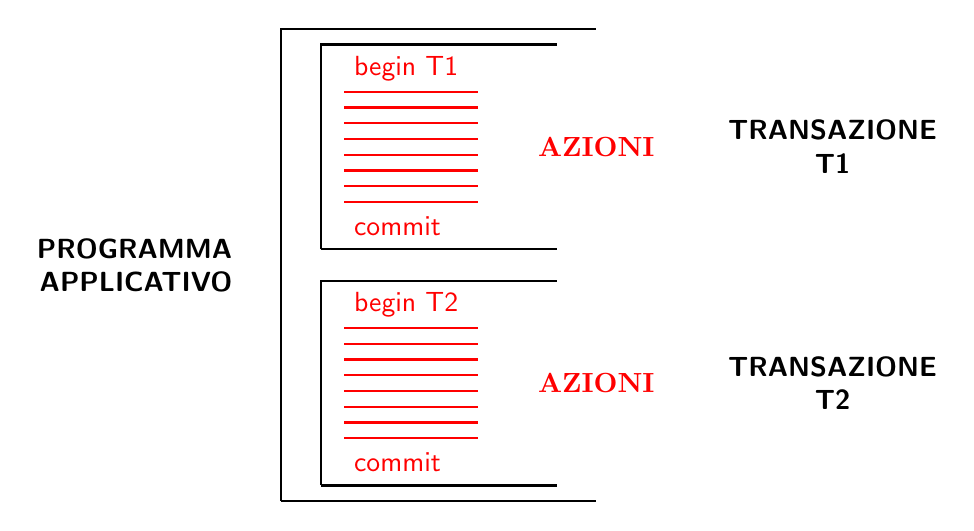
\begin{tikzpicture}[font=\sffamily]
% Program container
\draw[thick] (0, 0) -- (0, 6) -- (4, 6);
\draw[thick] (0, 0) -- (4, 0);
\node[anchor=east, align=right] at (-0.5, 3) {\textbf{PROGRAMMA}\\\textbf{APPLICATIVO}};

% Transaction 1
\draw[thick] (0.5, 3.2) -- (0.5, 5.8) -- (3.5, 5.8);
\draw[thick] (0.5, 3.2) -- (3.5, 3.2);
\node[text=red, anchor=west] at (0.8, 5.5) {begin T1};
\foreach \y in {3.8, 4.0, 4.2, 4.4, 4.6, 4.8, 5.0, 5.2} {
    \draw[red, thick] (0.8, \y) -- (2.5, \y);
}
\node[text=red, anchor=west] at (0.8, 3.5) {commit};
\node[text=red, font=\bfseries] at (4, 4.5) {AZIONI};
\node[align=center] at (7, 4.5) {\textbf{TRANSAZIONE}\\\textbf{T1}};

% Transaction 2
\draw[thick] (0.5, 0.2) -- (0.5, 2.8) -- (3.5, 2.8);
\draw[thick] (0.5, 0.2) -- (3.5, 0.2);
\node[text=red, anchor=west] at (0.8, 2.5) {begin T2};
\foreach \y in {0.8, 1.0, 1.2, 1.4, 1.6, 1.8, 2.0, 2.2} {
    \draw[red, thick] (0.8, \y) -- (2.5, \y);
}
\node[text=red, anchor=west] at (0.8, 0.5) {commit};
\node[text=red, font=\bfseries] at (4, 1.5) {AZIONI};
\node[align=center] at (7, 1.5) {\textbf{TRANSAZIONE}\\\textbf{T2}};

\end{tikzpicture}
\end{center}
\vspace{1em}

\section{Gestione Operativa delle Transazioni in JDBC e SQL}

La traduzione dei concetti transazionali nella pratica della programmazione avviene attraverso apposite API e sintassi del linguaggio di interrogazione.

\subsection{Transazioni in JDBC}
Nell'interfaccia Java Database Connectivity (JDBC), la scelta della modalità transazionale è demandata a un metodo specifico definito all'interno dell'interfaccia \texttt{Connection}: il metodo \texttt{setAutoCommit(boolean autoCommit)}.

\begin{itemize}
    \item Impostando \texttt{con.setAutoCommit(true)}, che rappresenta il comportamento di default dei driver JDBC, si attiva la modalità \textit{"autocommit"}. In questo scenario, il DBMS tratta ogni singola operazione SQL come se fosse una transazione autonoma a sé stante, implicitamente avviata ed immediatamente confermata al termine dell'istruzione.
    \item Impostando \texttt{con.setAutoCommit(false)}, si disabilita l'automatismo e si passa alla gestione esplicita delle transazioni via codice (da programma). In questa modalità si adoperano i metodi \texttt{con.commit()} per validare il blocco e \texttt{con.rollback()} per annullarlo.
\end{itemize}

È degno di nota che in JDBC non esiste un corrispettivo esplicito del comando di inizio transazione (nessuno \texttt{start transaction}). Il sistema adotta una convenzione implicita: una nuova transazione viene aperta automaticamente in due specifici momenti logici, ovvero all'atto dell'apertura iniziale della connessione verso il database e contestualmente all'esecuzione di un \texttt{commit} o \texttt{rollback} che ha sancito la conclusione della transazione immediatamente precedente.

\subsection{Transazioni nel linguaggio SQL}
Similmente a JDBC, nel puro linguaggio SQL una transazione inizia automaticamente al momento del primo comando SQL inoltrato dopo aver stabilito la "connessione" alla base di dati, oppure immediatamente dopo la conclusione della transazione precedente. Benché lo standard internazionale SQL indichi formalmente l'esistenza di un comando \texttt{start transaction}, questo è storicamente catalogato come opzionale. Ne consegue che molti motori relazionali non ne prevedano un utilizzo strettamente obbligatorio, sebbene RDBMS moderni ed estesi come PostgreSQL lo supportino e lo implementino regolarmente.

Per la conclusione della transazione, lo standard SQL impone:
\begin{itemize}
    \item \texttt{commit [work]}: impone al motore relazionale che tutte le operazioni specificate, conteggiate a partire dal momento esatto dell'inizio della transazione, vengano materialmente ed effettivamente eseguite sulla base di dati, divenendo visibili agli altri utenti e permanenti.
    \item \texttt{rollback [work]}: impone che si rinunci categoricamente all'esecuzione di tutte le operazioni specificate e accumulate dopo l'inizio della transazione. Qualsiasi alterazione pendente viene istantaneamente scartata.
\end{itemize}
Allo stesso modo di JDBC, molti sistemi relazionali offrono a livello di console o driver nativo la modalità \textit{autocommit}, in cui ciascuna istruzione isolata forma ed esaurisce l'intero ciclo di vita di una transazione.

\subsection{Esempi in codice SQL}
Per rendere evidente la sintassi descritta, si esamini un caso base di trasferimento di 10 unità monetarie da un conto a un altro.

\begin{verbatim}
start transaction;   -- (opzionale a seconda del DBMS)
update ContoCorrente
    set Saldo = Saldo + 10 where NumConto = 12202;
update ContoCorrente
    set Saldo = Saldo - 10 where NumConto = 42177;
commit;
\end{verbatim}

Le transazioni non sono semplici elenchi sequenziali di operazioni; esse incapsulano anche complessi rami condizionali. Si supponga di voler condizionare l'aggiornamento a un controllo sulla capienza residua del conto. Una volta decurtati i 10 dal conto origine (\texttt{NumConto = 42177}), il programma estrarrà il nuovo saldo transitorio all'interno della medesima transazione, per prendere una decisione (decision-making intrinsecamente atomico):

\begin{verbatim}
start transaction;
update ContoCorrente
    set Saldo = Saldo + 10 where NumConto = 12202;
update ContoCorrente
    set Saldo = Saldo - 10 where NumConto = 42177;

select Saldo into A
from ContoCorrente
where NumConto = 42177;

if (A >= 0) then commit
else rollback;
\end{verbatim}

La potenza del paradigma si esplica nell'istruzione condizionale: solo se il saldo post-operazione risulta non negativo ($A \geq 0$) le azioni vengono consolidamente persistite (\texttt{commit}); viceversa, invocando il \texttt{rollback}, il DBMS provvederà in autonomia a ripristinare sia il conto destinatario (\texttt{12202}) che quello mittente (\texttt{42177}) allo stato esatto che detenevano prima del comando \texttt{start transaction}.

\section{Le Proprietà Acide (ACID) delle Transazioni}

L'efficacia concettuale di una transazione risiede nel suo configurarsi come un'unità di elaborazione che gode invariabilmente delle cosiddette proprietà "ACIDE". L'acronimo, universalmente accettato in letteratura informatica, riassume i concetti di Atomicità, Consistenza, Isolamento e Durabilità (o persistenza). Ognuna di queste proprietà risponde a un'esigenza specifica dell'elaborazione di dati in ambienti critici e condivisi.

\subsection{Atomicità}

L'atomicità asserisce che una transazione rappresenta un'entità di elaborazione atomica, governata dalla legge del "tutto o niente". Questo principio si traduce nel fatto che se viene invocato ed eseguito il \texttt{commit}, allora \textit{tutte} le azioni programmate all'interno della transazione hanno effetto irrevocabile sullo stato finale della base di dati. Al contrario, se per qualsiasi ragione interviene un \texttt{abort} (o \texttt{rollback}), \textit{nessuna} azione sortisce effetto alcuno sul database persistito. Fondamentale per l'atomicità è che per il sistema non è logicamente e fisicamente ammissibile una terza possibilità: non può esistere in maniera visibile alcuno stato intermedio, ibrido o parzialmente aggiornato.

L'esito di una transazione può dipendere da varie cause, categorizzabili metaforicamente in:
\begin{itemize}
    \item \textbf{Commit}: costituisce la conclusione definita "naturale" e corretta del processo, in cui tutte le logiche si sono dipanate senza errori semantici o impedimenti di sistema.
    \item \textbf{Abort (Rollback)}: interrompe l'esecuzione e inverte gli effetti. Viene pittorescamente distinto in:
    \begin{itemize}
        \item \textbf{Suicidio}: l'abort richiesto esplicitamente dal codice dell'applicazione stessa (es. il controllo del saldo in rosso menzionato in precedenza). L'applicativo deduce un'anomalia logica e innesca autonomamente la rinuncia alle operazioni.
        \item \textbf{Omicidio}: l'abort imposto dall'alto, richiesto d'imperio dal sistema relazionale per preservare l'integrità. Questo fallimento indotto dal DBMS accade a seguito di circostanze non imputabili al flusso di istruzioni dell'utente: una rottura fisica (crash) del nodo, una violazione dei vincoli di integrità del modello relazionale, la risoluzione di un vicolo cieco causato dal controllo della concorrenza (deadlock), oppure uno stato di incertezza irreversibile in caso di fallimenti distribuiti.
    \end{itemize}
\end{itemize}

Per assicurare meccanicamente la garanzia del "tutto o niente", l'architettura di un RDBMS deve possedere la facoltà di cancellare a ritroso eventuali scritture provvisorie già annotate (operazione di \texttt{undo}) o di reinserirle post-crash (operazione di \texttt{redo}). Questi complessi recuperi di stato sono gestiti internamente dal DBMS e dai suoi moduli, sollevando integralmente l'utente e il programmatore dalla responsabilità di scriverne la logica nei propri applicativi.

\paragraph{Esempio di Atomicità in PostgreSQL.}
Per chiarire empiricamente questi esiti, si propone una casistica in ambiente PostgreSQL (da testare idealmente mediante l'utilizzo in parallelo di due sessioni client distinte per percepirne gli effetti in tempo reale).
Si predisponga un rudimentale schema relazionale con due tabelle \texttt{r1} e \texttt{r2}, legate tra loro da un vincolo di chiave esterna.

\begin{verbatim}
drop table if exists r1 cascade;
drop table if exists r2 cascade;
create table r1 (a integer primary key, b integer, c integer);
create table r2 (d integer primary key, e integer, f integer);
alter table r1 add constraint r1_c_fk
    foreign key (c) references r2 (d);
\end{verbatim}

\begin{itemize}
    \item \textbf{Operazione in autocommit:}
    Eseguendo una singola direttiva DML:
    \begin{verbatim}
    insert into r2 values (0,0,0);
    \end{verbatim}
    Il sistema avvia l'operazione in autocommit, e senza bisogno di delimitatori la riga viene persistentemente salvata nel dizionario di \texttt{r2}.

    \item \textbf{Transazione che abortisce:}
    Se si avvia esplicitamente il blocco con lo scopo di annullarlo:
    \begin{verbatim}
    start transaction;
    insert into r2 values (1,1,1);
    select * from r2;   -- La riga [1,1,1] risulterà visibile limitatamente
                        -- allo scope di questo blocco isolato.
    rollback;
    \end{verbatim}
    Al termine del \texttt{rollback}, la tabella ritornerà istantaneamente priva del record contenente i valori $(1,1,1)$. Il tentativo di tracciamento risulta estirpato senza lasciare alcuna traccia.

    \item \textbf{Transazione che va in commit:}
    Per terminare in modo coerente e definitivo una catena d'azione:
    \begin{verbatim}
    start transaction;
    insert into r2 values (1,1,1);
    insert into r1 values (1,1,1);
    commit;
    \end{verbatim}
    Al comando finale, il blocco di due istruzioni (corretto rispetto alla dipendenza gerarchica) viene solidificato nella base di dati a vantaggio di tutti gli attori che vi accedono.

    \item \textbf{Transazione incompleta (effetto di un crash):}
    Un'operazione intrapresa senza poterla concludere:
    \begin{verbatim}
    start transaction;
    insert into r2 values (2,2,2);
    \end{verbatim}
    Se in questo momento esatto si procede ad "uccidere pgadmin" (simulando un severo crash dell'applicativo o della connessione senza inviare abort espliciti), la transazione risulta spezzata e diviene orfana. Il DBMS interpreterà il disallineamento come fallimentare e provvederà autonomamente tramite procedure di recupero (recovery) ad abbattere lo stato provvisorio, applicando di fatto un abort (omicidio di sistema).
\end{itemize}

\subsection{Consistenza}

La proprietà di Consistenza stabilisce che la transazione deve rigorosamente rispettare e validare i vincoli di integrità del modello dei dati associati alle relazioni. Questa correttezza impone che, dato uno stato iniziale corretto prima dell'invocazione della transazione (prerequisito assunto come vero), anche lo stato finale, al termine della procedura transazionale, debba risultare inoppugnabilmente corretto e congruente rispetto allo schema logico. Se lo stato finale computato non rispetta in toto le restrizioni definite sul database, l'intero blocco fallisce inesorabilmente causando un'eccezione abortiva.

La peculiarità architetturale della Consistenza risiede nel fatto che, durante l'esecuzione vera e propria delle istruzioni, il sistema può ammettere la violazione di un vincolo. Nelle basi di dati transazionali, i vincoli di integrità sono di norma analizzati e controllati sistematicamente per ciascuna operazione isolata DML. Viene tuttavia concessa a livello DDL la possibiltà architetturale di definire il concetto di "vincolo differito" (deferred constraint): tale meccanismo sospende la verifica tassativa del requisito referenziale o di entità fino all'attimo conclusivo di emissione del \texttt{commit}.

\paragraph{Il problema del vincolo rigido (Immediato).}
Osserviamo nuovamente PostgreSQL, utilizzando l'impianto base descritto in precedenza per la definizione logica:

\begin{verbatim}
drop table if exists r1; drop table if exists r2;
create table r1 (a integer primary key, b integer, c integer);
create table r2 (d integer primary key, e integer, f integer);
alter table r1 add constraint r1_c_fk
    foreign key (c) references r2 (d);
\end{verbatim}

Tentando di popolare il dataset, si simula l'apertura di un pacchetto di esecuzione:
\begin{verbatim}
start transaction;
insert into r1 values (3,3,3);
\end{verbatim}
Questa singola istruzione fallisce repentinamente. Il comportamento è dettato dalla natura immediata del vincolo: per memorizzare il valore $c=3$ in \texttt{r1}, il relazionale esige pedissequamente che la tupla con $d=3$ esista già in \texttt{r2}. Il vincolo viene valutato immediatamente, rigettando prematuramente la tupla.

\paragraph{Vincolo Differito (Deferred constraint).}
Si modifichi il DDL del database introducendo esplicitamente la direttiva di procrastinazione:
\begin{verbatim}
rollback;
drop table if exists r1; drop table if exists r2;
create table r1 (a integer primary key, b integer, c integer);
create table r2 (d integer primary key, e integer, f integer);
alter table r1 add constraint r1_c_fk
    foreign key (c) references r2 (d)
    deferrable initially deferred;
\end{verbatim}
Eseguendo ora la casistica difettosa mostrata poc'anzi:
\begin{verbatim}
start transaction;
insert into r1 values (3,3,3);
commit;
\end{verbatim}
In questo scenario, il DBMS accetta formalmente e processa la prima istruzione \texttt{insert} (anche se essa genera una temporanea orfanità logica), senza lanciare eccezioni. Tuttavia, nel momento esatto in cui viene impartito il \texttt{commit}, il \textit{Gestore dell'integrità a tempo di esecuzione} entra in scena controllando tutti gli arretrati; constatando la definitiva mancanza del nodo primario su \texttt{r2}, la transazione fallisce rovinosamente proprio nell'attimo del salvataggio.

Per concretizzare una chiusura consistente occorrerà fornire i dati in maniera olisticamente completa:
\begin{verbatim}
start transaction;
insert into r1 values (3,3,3);
insert into r2 values (3,3,3);
commit;
\end{verbatim}
Questo secondo flusso restituisce esito "\textit{Ok!}": alla richiesta di chiusura differita, il motore rileva che, seppur momentaneamente mancante dopo la prima \texttt{insert}, il record genitore $d=3$ in \texttt{r2} è stato infine materializzato tramite la seconda \texttt{insert}. Lo stato finale complessivo è concorde con i domini del DBMS.

\paragraph{Perché differire i vincoli? Il caso necessario.}
Esistono circostanze complesse, specificamente nei \textbf{cicli di vincoli di integrità referenziale}, in cui la procrastinazione del controllo costituisce l'unica via tecnicamente percorribile. Si supponga un paradigma bidirezionale puro (chiken-and-egg problem) dove le entità si richiamano in modo circolare:

\begin{verbatim}
drop table if exists r1; drop table if exists r2;
create table r1 (a integer primary key, b integer, c integer);
create table r2 (d integer primary key, e integer, f integer);

alter table r1 add constraint r1_c_fk
    foreign key (c) references r2(d);
alter table r2 add constraint r2_c_fk
    foreign key (f) references r1(a);
\end{verbatim}
Tentando un inserimento standard:
\begin{verbatim}
start transaction;
insert into r1 values (3,3,3);
insert into r2 values (3,3,3);
commit;
\end{verbatim}
Questo approccio produrrà inesorabilmente un errore al primo rigo, rendendo impensabile qualsiasi sequenza inseritiva: non posso caricare dati in \texttt{r1} se manca l'aggancio in \texttt{r2}, ma in via speculare, non posso caricare neppure su \texttt{r2} in assenza del relativo punto d'appoggio primario in \texttt{r1}. I due vincoli sono intrinsecamente paralizzanti.
L'adozione della clausola \texttt{deferrable initially deferred} su entrambi i constraints consente di sospendere artificialmente la semantica relazionale: si inietta la tupla in \texttt{r1}, successivamente quella di chiusura in \texttt{r2}, e, una volta invocato il controllo unico al \texttt{commit}, il grafo si presenterà simmetricamente ed integralmente consistente ("\textit{Ok!}").

\subsection{Isolamento}

L'isolamento prescrive che l'esecuzione di una determinata transazione non deve in alcun caso risentire degli effetti scaturiti dallo svolgimento di altre transazioni concorrenti presenti nel medesimo sistema. Detto in altri termini, l'esecuzione concorrente e intrecciata (interleaved) di una vasta collezione di transazioni, governata dallo scheduler del motore relazionale, deve poter produrre un risultato logicamente identico a quello che si sarebbe materializzato se si fosse forzata una rigidissima esecuzione sequenziale (seriale). Le operazioni devono verificarsi \textit{come se}, per un qualsivoglia processo transazionale in corso d'opera, tutte le altre elaborazioni fossero virtualmente inesistenti o sospese.

I due postulati fondamentali che sorreggono l'isolamento sono:
\begin{enumerate}
    \item La protezione da corruzioni dati quali incroci tra due operazioni quasi contestuali (es. due prelievi asincroni descritti nell'introduzione).
    \item La protezione e occultamento totale dei risultati intermedi. I dati temporaneamente calcolati o scritti in seno a una transazione viva non debbono per nessuna ragione poter essere visibili agli altri client connessi prima della conclusione della medesima. Qualora l'infrastruttura disattendesse questo principio vitale (permettendo la cosiddetta "dirty read" o lettura sporca), le transazioni terze potrebbero utilizzare e veicolare all'esterno informazioni sbagliate. Di conseguenza, qualora la transazione originaria dovesse andare in abort volontario o cadere per crash, occorrerebbe annullare forzatamente anche tutte le transazioni che nel frattempo hanno consumato quei dati temporanei, generando una disastrosa propagazione di invalidamenti sistemici, tristemente nota nella teoria dei database come "\textbf{effetto domino}" (cascading rollbacks).
\end{enumerate}

\paragraph{Meccanica dell'isolamento e blocchi.}
Il sistema preserva l'integrità introducendo meccanismi di blocco temporaneo dei record (locking).
Prendiamo in esame una contesa esplicita simulabile ricorrendo a due Client disgiunti e concorrenti:

\begin{itemize}
    \item \textit{Stato Iniziale:}
    \begin{verbatim}
    drop table if exists r2 cascade;
    create table r2 (d integer primary key, e integer, f integer);
    insert into r2 values (1,1,1);
    \end{verbatim}

    \item \textit{Evoluzione del Client 1:}
    Il primo utente apre le danze transazionali richiedendo una prima alterazione in lettura-scrittura sul dominio per $d=1$:
    \begin{verbatim}
    start transaction;
    update r2 set e = e + 1 where d = 1;
    select * from r2;
    \end{verbatim}
    In questo esatto frangente il Client 1 riceverà a video il dato proiettato temporaneamente nel buffer, in cui il campo $e$ vale $2$. La riga soggiacente nel disco è stata acquisita in modalità esclusiva (lock in scrittura).

    \item \textit{Evoluzione concorrente del Client 2:}
    Contemporaneamente, da terminale parallelo, l'utente due avvia la propria procedura di modifica:
    \begin{verbatim}
    start transaction;
    select * from r2;
    update r2 set e = e + 10 where d = 1;
    \end{verbatim}
    Il Client 2 eseguirà indenne la pura istruzione \texttt{select} prima del lock (visualizzando l'originale $e=1$), ma l'esecuzione dell'istruzione \texttt{update} non si compirà immantinente: l'isolamento del sistema provocherà l'entrata in uno stato di attesa silente e indefinita (sospensione o blocco). Il Client 2 non è distrutto, ma temporaneamente paralizzato poiché la risorsa associata al predicato $d=1$ risulta contesa ed in possesso del Client 1, il quale non ha ancora certificato se le proprie variazioni si tramuteranno o meno in una modifica globale.
\end{itemize}

Questo stallo concorrenziale permane finché il Client 1 non assume una determinazione sulla propria chiusura:
\begin{itemize}
    \item \textbf{Scenario di Commit:} Il Client 1 invia un \texttt{commit}. L'aggiornamento transitorio si trasforma in uno stato di consistenza formale, il lucchetto di locking decade ed il DBMS risveglia il Client 2, permettendo al suo applicativo bloccato di terminare regolarmente la propria \texttt{update} (sommando $+10$ su quello che ora diviene il nuovo valore confermato di $e=2$, giungendo quindi a $e=12$). Anche il Client 2 concluderà a sua volta con un \texttt{commit}.
    \item \textbf{Scenario di Rollback:} Alternativamente, il Client 1 propende per scartare il progresso inserendo \texttt{rollback}. Nell'istante esatto dell'annullamento, il sistema "protegge" la risorsa cancellando il transitorio e ristabilendo il record alle condizioni antecedenti ($e=1$). Il lucchetto viene rilasciato. Immediatamente dopo, il Client 2, precedentemente sospeso, si sveglia e porta finalmente a termine il calcolo per cui era rimasto in pendenza applicando il suo differenziale alcolabile di $+10$ alla base $e=1$, stabilizzando logicamente e coerentemente la nuova riga a $e=11$ a seguito di proprio \texttt{commit}.
\end{itemize}

In entrambe le fattispecie l'approccio pessimistico di immobilizzazione condizionale garantisce che l'esito formale corrisponda in tutto e per tutto ad un incasellamento strettamente sequenziale delle manovre.

\subsection{Durabilità (Persistenza)}

La Durabilità costituisce il suggello finale dell'architettura: essa decreta che tutti gli effetti prodotti dai mutamenti operati da una transazione, una volta andata esplicitamente a buon fine ed elaborata dal comando di \texttt{commit}, non andranno perduti sotto alcuna circostanza. Tali effetti permarranno registrati ("durano per sempre") ed incorruttibili dinanzi ad ogni futuro problema strutturale e ad una vastità di guasti. Nel gergo dell'amministrazione DB, il verbo "commit" perde l'accezione gergale per riappropriarsi del proprio rigore etimologico: esso attesta un severo e insindacabile "\textit{impegno}".

Nella prassi l'insidia più temuta per la preservazione permanente è celata nell'esistenza del \textit{buffer} ramificato. Avendo il motore elaborativo condotto calcoli unicamente in memoria temporanea ed appoggiandosi pesantemente su processi di scaricamento differito sul disco fisso (I/O logici e fisici), la manifestazione inattesa di un evento bloccante disastroso (un black out sistemico ad alta criticità) esporrebbe teoricamente l'infrastruttura al rischio catastrofico di dispersione irreversibile dei record che non sono ancora materialmente andati incontro al processo di immagazzinamento nel piatto ("scaricati" su disco). Onde prevenire in radice la probabilità di simili danni la durabilità fa ampio ricorso ai registri crittografici (log di affidabilità o log files) che trascrivono in maniera rigidamente sincrona le alterazioni validate transazionalmente prima di accreditare lo stato del \texttt{commit} applicativo medesimo.

\section{Transazioni Relazionate ai Moduli di un DBMS}

È opportuno chiudere il compendio mappando i criteri cardinali appena illustrati in riferimento alle sub-architetture e al diagramma descritti nei precedenti capitoli introduttivi. Ognuna delle proprietà imposte dal paradigma ACID si incarna materialmente nel lavoro invisibile dei motori che governano il core del DBMS:

\begin{itemize}
    \item Le proprietà di \textbf{Atomicità} e \textbf{Durabilità} si collocano sotto l'egida esclusiva del \textbf{Gestore dell'affidabilità (Reliability manager)}. Ad esso spetta redigere ed interrogare i log, implementare le sofisticate e costose manovre di \textit{undo}/\textit{redo} nonchè sovrintendere alle policy del flush verso memoria secondaria in sinergia col gestore del buffer.
    \item La proprietà dell'\textbf{Isolamento} rientra storicamente nell'ambito e nelle competenze applicative del \textbf{Gestore della concorrenza}. Il compito immane di monitorare e dispiegare istanti per istante lucchetti relazionali e semafori sui diversi livelli di granularità risponde ad una sua esclusiva prerogativa schedulatrice.
    \item La proprietà di \textbf{Consistenza} è presidiata integralmente dal \textbf{Gestore dell'integrità a tempo di esecuzione}. Operando alle dipendenze dirette dei metadati creati preventivamente in ausilio con il costrutto ed il supporto vitale del compilatore del vocabolario strutturale DDL, esso valuta attivamente scostamenti, vincoli incrociati e, non di meno, posticipazioni temporali (i meccanismi \textit{deferrable}) in totale trasparenza e autonomia.
\end{itemize}
